\documentclass[a4paper, 11pt]{article}
\usepackage{fullpage}
\usepackage{mathtools, nccmath}
\usepackage{graphicx}
\usepackage{float}
\usepackage{amsmath}
\renewcommand{\figurename}{Fig.}
\renewcommand{\refname}{Bibliografia}


\begin{document}
%Header
\noindent
\large\textbf{Corso di Metodi di Ottimizzazione} \hfill \textbf{Gruppo E} \\
\normalsize A.A. 2018/2019 \hfill Ing. Saverio Del Prete \\
Prof. Raffaele Martone \hfill Ing. Bernardo Giordano \\
\hphantom{}\hfill Ing. Lucia Migliaccio

\section*{Traccia del problema}

Progetto ottimo di un campo magnetico con incognite geometriche e di corrente di
una spira.

\section*{Descrizione del sistema fisico}

Il sistema è composto da un certo numero di spire simmetriche (supporremo $n=6$)
concentriche rispetto allo stesso asse $z$. I parametri di progetto, ovvero
posizione, raggio e intensità di corrente, sono noti per tutte le spire tranne
che per una coppia.

\begin{figure}[H]
	\centering
	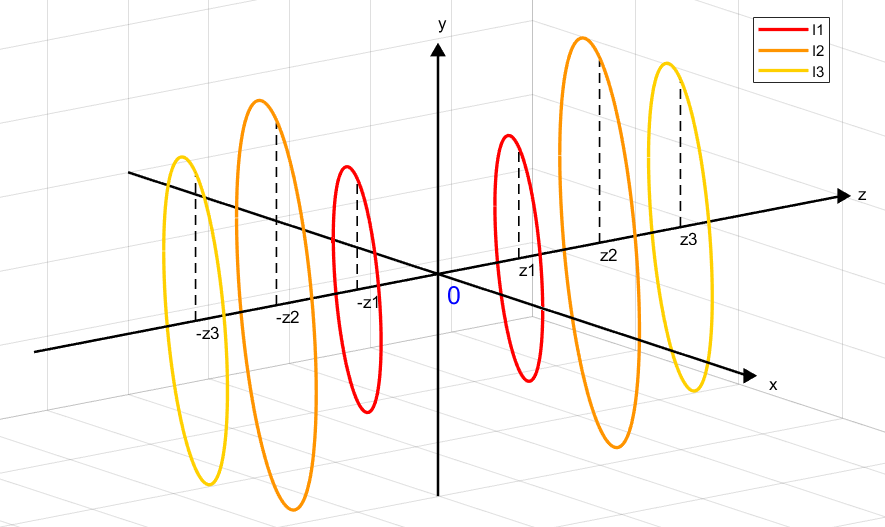
\includegraphics[width=12cm]{assets/figure1}
	\caption{Sistema fisico posizionato nel piano $xyz$.}
\end{figure}

\noindent
Il campo magnetico generato dalla corrente circolante nelle spire può essere
valutato sull’asse utilizzando la legge di Biot-Savart. La legge di Biot-Savart
ci permette di valutare il campo magnetico B prodotto in un punto dello spazio
da una spira percorsa da corrente elettrica.

\begin{figure}[H]
	\centering
	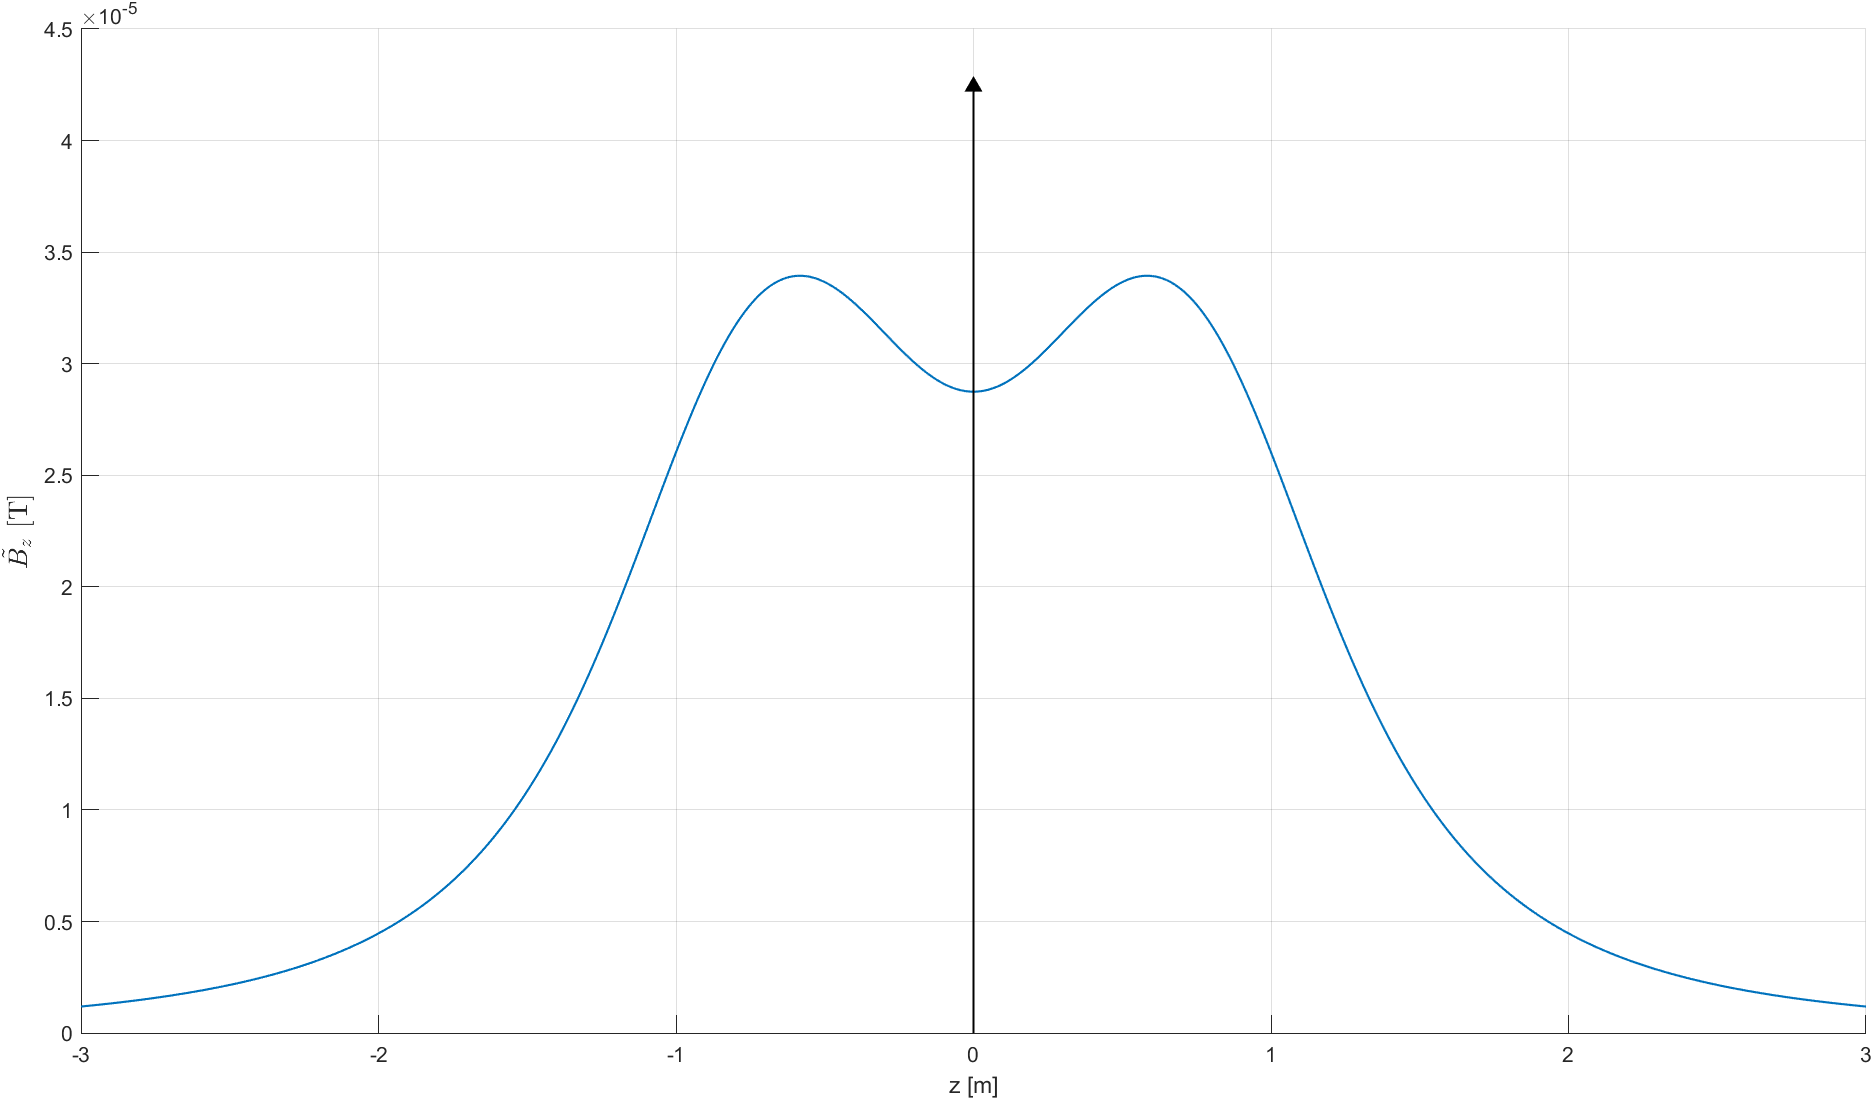
\includegraphics[width=10cm]{assets/figure2}
	\caption{Schema di una spira concentrica all'asse $z$.}
\end{figure}

\noindent
Il campo magnetico sull’asse $z$  di una spira caratterizzata da una corrente
$I$, lunghezza $L$, raggio $R$ e posizione $Z$ (supponiamo, per
semplicità, posizionata in $Z=0$), si valuta come
\[dB_{z}=\frac{\mu_{0}IdL}{4\pi}\frac{R}{\left(z^{2}+R^{2}\right)^{3/2}}\]
dove $\mu_{0}$ è la permeabilità magnetica nel vuoto, $\mu_{0}=4{\pi}10^{-7}
H/m$. \\
L’integrale di $dL$ risulta essere proprio la circonferenza della spira, ovvero
$2{\pi}R$. Integrando quindi, si ricava la funzione del campo magnetico
sull'asse
\[B_{z}=\frac{\mu_{0}}{4\pi}\frac{2{\pi}R^{2}I}{\left(z^{2}+R^{2}\right)^{3/2}}=\frac{\mu_{0}}{2}\frac{R^{2}I}{\left(z^{2}+R^{2}\right)^{3/2}}\]
Siano $Z_{i}$, $R_{i}$ e $I_{i}$ rispettivamente la posizione, il raggio e la
corrente relative alla spira $i$-esima. \\
Sia inoltre $n=6$ il numero complessivo delle spire facenti parte del sistema.
Considerando adesso la sovrapposizione degli effetti di tutte le spire del
sistema e tenendo presente che le spire sono simmetriche rispetto al piano $xy$,
il campo magnetico complessivo sull’asse $z$ varrà

\begin{align*}
	B_{z}
		&=\frac{\mu_{0}}{4{\pi}}\left(\sum_{i=1}^{n/2}\frac{2{\pi}I_{i}R_{i}^{2}}{\left(\left(Z_{i}-z\right)^{2}+R_{i}^{2}\right)^{3/2}}+\frac{2{\pi}I_{i}R_{i}^{2}}{\left(\left(Z_{i}+z\right)^{2}+R_{i}^{2}\right)^{3/2}}\right)\\
		&=\frac{\mu_{0}}{2}\left(\sum_{i=1}^{n/2}\frac{I_{i}R_{i}^{2}}{\left(\left(Z_{i}-z\right)^{2}+R_{i}^{2}\right)^{3/2}}+\frac{I_{i}R_{i}^{2}}{\left(\left(Z_{i}+z\right)^{2}+R_{i}^{2}\right)^{3/2}}\right)
\end{align*}
\noindent
L'obiettivo del progetto della spira mancante risulta essere la migliore
approssimazione di un campo magnetico avente la seguente caratteristica

\begin{figure}[H]
	\centering
	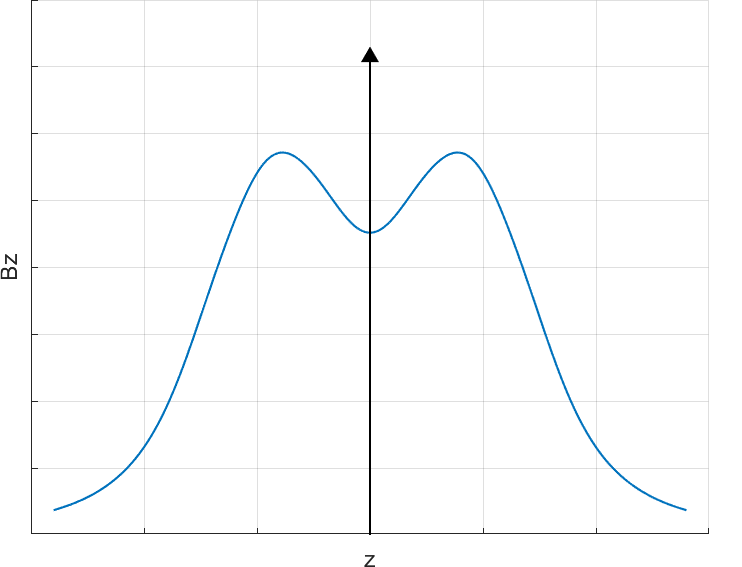
\includegraphics[width=10cm]{assets/figure3}
	\caption{Campo magnetico sull'asse $z$ desiderato.}
\end{figure}
\noindent
Sia adesso $B_{z}$ il campo magnetico generato dalla sovrapposizione delle spire
del sistema da progettare, e $\tilde{B_{z}}$ il campo magnetico desiderato. Al
fine da ottenere una discrepanza più piccola possibile, è di nostro interesse lo
studio della funzione
\[||B_{z}-\tilde{B_{z}}||\] dove $B_{z}$ è la funzione del campo magnetico da
progettare e $\tilde{B_{z}}$ è quella del campo desiderato. \\
Siccome i parametri di progetto delle spire 1 e 3 (e, quindi, delle rispettive
spire simmetriche) sono noti ed esattamente uguali a quelli del sistema
desiderato, la suddetta differenza in norma si scriverà come

\begin{equation}
	\begin{split}
	||B_{z}-\tilde{B_{z}}||
		=& \Bigl|\Bigl|\frac{\mu_{0}}{2}(\frac{I_{2}R_{2}^{2}}{((Z_{2}-z)^{2}+R_{2}^{2})^{3/2}}+\frac{I_{2}R_{2}^{2}}{((Z_{2}+z)^{2}+R_{2}^{2})^{3/2}})- \\
		 & \frac{\mu_{0}}{2}(\frac{\tilde{I_{2}}\tilde{R_{2}}^{2}}{((\tilde{Z_{2}}-z)^{2}+\tilde{R_{2}}^{2})^{3/2}}+\frac{\tilde{I_{2}}\tilde{R_{2}}^{2}}{((\tilde{Z_{2}}+z)^{2}+\tilde{R_{2}}^{2})^{3/2}})\Bigr|\Bigr| \\
		=& \frac{\mu_{0}}{2}\Bigl|\Bigl|\frac{I_{2}R_{2}^{2}}{((Z_{2}-z)^{2}+R_{2}^{2})^{3/2}}+\frac{I_{2}R_{2}^{2}}{((Z_{2}+z)^{2}+R_{2}^{2})^{3/2}}- \\
		 & \frac{\tilde{I_{2}}\tilde{R_{2}}^{2}}{((\tilde{Z_{2}}-z)^{2}+\tilde{R_{2}}^{2})^{3/2}}+\frac{\tilde{I_{2}}\tilde{R_{2}}^{2}}{((\tilde{Z_{2}}+z)^{2}+\tilde{R_{2}}^{2})^{3/2}}\Bigr|\Bigr|
	\end{split} 
\end{equation}
\noindent
% da aggiustare
Possiamo dunque considerare la 1 come \emph{la funzione di costo} del nostro problema.

\section*{Normalizzazione e funzione di costo}

La normalizzazione è l'operazione che dato un vettore lo porta ad avere una
norma unitaria. Possiamo normalizzare rispetto al rapporto $\frac{\mu_{0}}{2}$,

% su cosa cazzo normalizziamo?  
\section*{Analisi dei parametri}


\section* {Ricerca del minimo}

L'algoritmo di ricerca del minimo fa uso del concetto di simplesso, cioè un politopo di N+1 vertici 
in N dimensioni, ovvero: un segmento di retta in una dimensione, un triangolo in due 
dimensioni, un tetraedro in tre dimensioni. Il metodo ci permette di limitare la
ricerca della soluzione ottima ai vertici del politopo. La ricerca avviene 
attraverso il movimento del politopo, il politopo può:\\   
-Ribaltarsi:    valuto il valore della funzione nei 3 vertici, idividuo il vertice
	con il valore 'peggiore' tengo fermo gli altri due e ribalto quello 
	'peggiore' a banda opposta(caso N=2). \\
-Contrarsi:     se un vertice del politopo rimane più a lungo di un numero 
	specifico di iterazioni M (M fissato) il politopo viene contratto.\\
Il simplesso è un metodo zero-th, ache se non faccio uso di derivate sto stimando in qualche
modo una direzione di discesa.


\begin{thebibliography}{9}
	% \bibitem{id}Author\emph{title}[online]. Editor.
\end{thebibliography}
\end{document}